\chapter{Implementationsdetails}
\label{chap:implementierung}
In diesem Kapitel werden die Funktionalitäten der Pipeline zusammengetragen. Um die Anforderungen genauer zu beschreiben, wird ein Use-Case-Diagramm und ein Flussdiagramm dargestellt und beschrieben. Zudem werden konkrete funktionale und nichtfunktionale Anforderungen des Systems erfasst. Abschließend werden verwendete Technologien und Implementationsaspekte genauer beschrieben.
\section{Beschreibung des entwickelten Systems}
\label{sec:beschreibungsystem}
Es wird eine Lösung gesucht, die eine effiziente Verarbeitung von \emph{Bedarfsmeldungen} durchführen kann. Welche Aspekte in einer Bedarfsmeldung relevant sind, wurde bereits im Kapitel \ref{chap:erwartungshaltung} näher erläutert. Auf Basis welcher Methodiken und Ansätze die relevanten Informationen extrahiert werden können, wurde in Kapitel \ref{sec:literaturueberblick} dargestellt. Nun gilt es eine Lösung zu entwickeln, die diese Ansätze in einem System implementiert und Möglichkeiten zur Evaluation bietet. Die Idee ist es, eine Pipeline zu entwickeln, die Möglichkeiten zum laden von \emph{Bedarfsmeldungen} bietet. Damit alle Ansätze und Methoden zur Extraktion von Informationen gut funktionieren und vergleichbar bleiben, wird eine Übersetzungsfunktion der \emph{Bedarfsmeldungen} benötigt. Auch wenn die \emph{Bedarfsmeldungen} in den meisten Fällen auf Deutsch sind, hilf es diese zu übersetzen, damit keine Unterschiede in der Ergebnisqualität resultiert, da einige Methoden und Ansätze auf Basis von Englischen Trainingssätzen trainiert wurden. Schließlich müssen alle aus Kapitel \ref{sec:literaturueberblick} untersuchten Ansätze implementiert und nutzbar sein. Sie sollen die Möglichkeit haben \emph{Bedarfsmeldungen} als Input zu erhalten und eine Ausgabe zurückzugeben. Zur besseren Evaluationsmöglichkeit soll das System modular sein, damit Methoden und Ansätze nach belieben durchgetauscht werden können. Zur Überprüfung der Laufzeit soll eine Zeitmessung verfügbar sein, die die Zeit zwischen dem Start und der Beendigung des Systems zurückgibt.\\

\todo{erzählen was die Pipeline leisten soll, im Falle vom Hybrid wird wahrscheinlich noch data-fusion gebraucht, vektorisierung eventuell auch noch für cosine similarity}
\newpage
\section{Use-Case}
\label{sec:usecase}
In diesem Kapitel werden die Interaktionen zwischen Benutzer und System beschrieben. Dazu wird ein Use-Case-Diagramm angefertigt, das eine grafische Übersicht über alle Anwendungsfälle bietet.
\begin{figure}[H]
	\centering  
	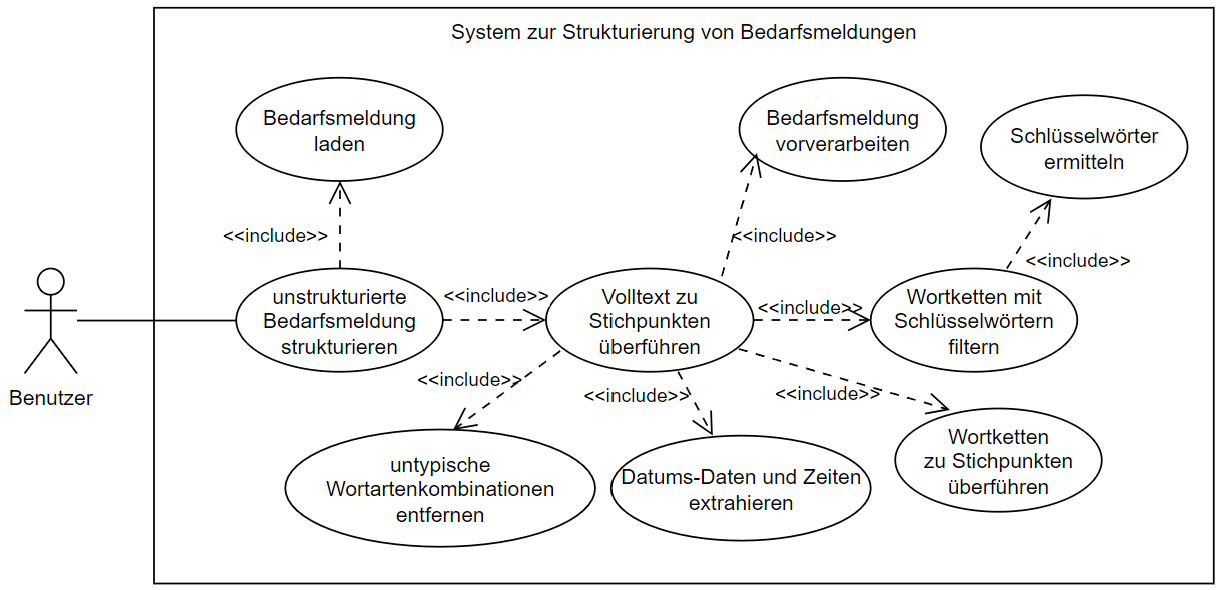
\includegraphics[width=\linewidth]{Abbildungen/use-case.png}
	\caption{Use-Case Diagramm der Pipeline.}
	\label{fig:usecasediagrammwirklich}
\end{figure}\mbox{} \\
In der Abbildung \ref{fig:usecasediagrammwirklich} ist das Use-Case Diagramm zur Pipeline. Es existiert ein Akteur. Dieser hat die Möglichkeit eine oder mehrere \emph{Bedarfsmeldungen} zu laden. Zudem kann diese ins Englische übersetzt werden. Darüber hinaus kann die \emph{Bedarfsmeldung} durch \emph{Preprocessing} vorverarbeitet werden und irrelevante Wörter und Zeichen aus der \emph{Bedarfsmeldung} ausschließen. Der Benutzer kann die Methoden \emph{TF-IDF}, \emph{TextRank}, \emph{N-Gram}, \emph{POS-Tagging} und \emph{NER} mit der \emph{Bedarfsmeldung} anwenden. Wenn mehrere Methoden in der Pipeline sind, können die Resultate durch die Anwendung von \emph{Data-Fusion} zusammengeführt werden.
\section{Anforderungen}
Im Folgenden werden die funktionalen sowie nichtfunktionalen Anforderungen des Systems beschrieben. Diese Informationen wurden aus der Beschreibung des Systems aus Kapitel \ref{sec:beschreibungsystem} und dem Use-Case aus Kapitel \ref{sec:usecase} hergeleitet und bilden den Rahmen des Systems.
\subsection{Funktionale Anforderungen}
Die funktionalen Anforderungen beschreiben konkrete Funktionalitäten des Systems. Dazu werden zusammengehörende Anforderungen nummeriert und im Falle der Systemanforderungen in detaillierte Unterpunkte aufgelistet und beschrieben.
\paragraph{Benutzeranforderungen}
\begin{enumerate}
	\item Dem Benutzer soll es möglich sein, Extraktionsmethoden austauschen zu können.
	\item Dem Benutzer soll es möglich sein, die Laufzeit des Systems zu sehen.
\end{enumerate}
\todo{vielleicht dann auch die evaluationsschritte einbauen}
\paragraph{Systemanforderungen}
\begin{enumerate}[label=1.\arabic*]
	\item Die \emph{Bedarfsmeldungen} sollen geladen werden können.
	\item Beim laden können eine oder mehrere \emph{Bedarfsmeldungen} geladen werden.
	\item Das System soll die Datenformate \emph{.txt} und \emph{.json} unterstützen.
\end{enumerate}
\begin{enumerate}[label=2.\arabic*]
	\item Die Bedarfsmeldungen sollen ins Englische übersetzt werden können.
\end{enumerate}
\begin{enumerate}[label=3.\arabic*]
	\item Das System soll Methoden des Preprocessing zur Bereinigung eines Volltextes implementiert haben.
	\item Das Preprocessing soll ein Volltext als Eingabe erhalten.
	\item Das Preprocessing soll den Volltext als Ausgabe zurückgeben.
\end{enumerate}
\begin{enumerate}[label=4.\arabic*]
	\item Das System soll die Methode \emph{TF-IDF} als Modul implementiert haben.
	\item Das Modul soll die Möglichkeit haben ein Volltextes als Eingabe für die implementierte Methode mitzugeben.
\end{enumerate}
\begin{enumerate}[label=5.\arabic*]
	\item Das System soll die Methode \emph{TextRank} als Modul implementiert haben.
	\item Das Modul soll die Möglichkeit haben ein Volltextes als Eingabe für die implementierte Methode mitzugeben.
\end{enumerate}
\begin{enumerate}[label=6.\arabic*]
	\item Das System soll die Methode \emph{N-Gram} als Modul implementiert haben.
	\item Das Modul soll die Möglichkeit haben ein Volltextes als Eingabe für die implementierte Methode mitzugeben.
\end{enumerate}
\begin{enumerate}[label=7.\arabic*]
	\item Das System soll die Methode \emph{POS-Tagging} als Modul implementiert haben.
	\item Das Modul soll die Möglichkeit haben ein Volltextes als Eingabe für die implementierte Methode mitzugeben.
\end{enumerate}
\begin{enumerate}[label=8.\arabic*]
	\item Das System soll die Methode \emph{NER} als Modul implementiert haben.
	\item Das Modul soll die Möglichkeit haben ein Volltextes als Eingabe für die implementierte Methode mitzugeben.
\end{enumerate}
\begin{enumerate}[label=8.\arabic*]
	\item Das System soll die Möglichkeit haben die Laufzeit des Systems zu messen.
	\item Der Startzeitpunkt wird beim Systemstart festgehalten.
	\item Der Endzeitpunkt wird beim Systemstop festgehalten.
	\item Die Differenz aus dem Start- und Stop- Zeitpunkt wird ermittelt.
\end{enumerate}
\subsection{Nichtfunktionale Anforderungen}
Hierbei handelt es sich um qualitätsbezogene Anforderungen. Diese umfassen nicht konkrete Funktionen des Systems, sondern stellen Rahmenbedingungen des Systems im Ganzen zusammen.
\begin{enumerate}
	\item Das System soll modular aufgebaut sein, um die Extraktionsmethoden austauschen zu können.
	\item Das System soll in der Lage sein, mehrere \emph{Bedarfsmeldungen} laden zu können.
\end{enumerate}
\newpage
\section{Systemablauf}
\todo{Flussdiagramm beschreiben und in der Einleitung nicht vergessen im Ablauf anzupassen dass das kein Klassendiagramm mehr ist}
\begin{figure}[H]
	\centering  
	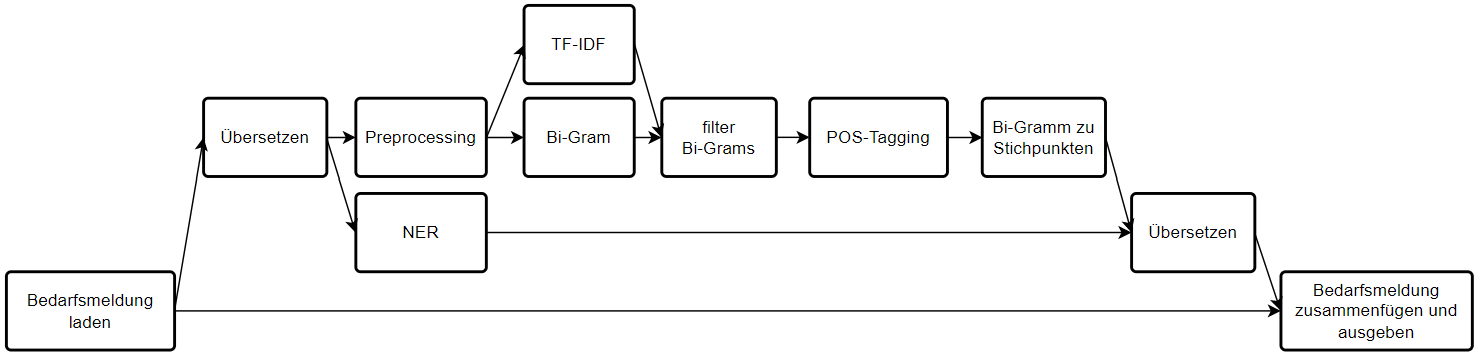
\includegraphics[width=\linewidth]{Abbildungen/flowchart.png}
	\caption{Flussdiagramm der Pipeline.}
	\label{fig:flowchart}
\end{figure}\mbox{} \\
\section{Details zur Implementierung der Pipeline}
Dieses Kapitel beschreibt den technischen Entwicklungsprozess zur Umsetzung der Anforderungen des Systems. Die Implementierung fokussiert sich auf die Umsetzungen von Technologien und Funktionsweisen verschiedener Anforderungen. Zudem wird die Struktur des Projektes aufgezeigt.
\subsection{Umsetzung}
Die Pipeline wurde in der Programmiersprache Python umgesetzt. Python hat sich zu einer der populärsten interpretierten Programmiersprachen entwickelt \cite{mckinney2012python}. Die Programmiersprache eignet sich insbesondere für die Erstellung kleiner Programme und Skripte, die zur Automatisierung von Aufgaben eingesetzt werden können \cite{mckinney2012python}. Python hat eine große und aktive Community für wissenschaftliche Berechnungen und Datenanalysen hervorgebracht und hat sich in den letzten Jahren zu einer der wichtigsten Sprachen für Data Science, maschinelles Lernen und allgemeine Softwareentwicklung in Wissenschaft und Industrie entwickelt \cite{mckinney2012python}. Python unterstützt Modularität, wodurch ein Teil der Anforderungen somit abgedeckt werden kann. Das Ziel der Arbeit besteht nicht in der Erweiterung der Verfahren, sondern in der Evaluierung ihrer Eignung zur Extraktion relevanter Informationen aus \emph{Bedarfsmeldungen}. Dadurch erfolgt die Implementierung der Methoden aus den Anforderungen nicht manuell, sondern es wurde auf bereits existierende Bibliotheken zurückgegriffen.
\subsection{Projektstruktur}
\label{sec:projektstruktur}
Das Projekt wird in einem git Repository gespeichert und versioniert. Die Projektstruktur ist ohne zusätzliche Konfigurationsdateien wie folgt aufgebaut:
\dirtree{%
	.1 .git/.
	.2 modules/.
	.3 nGram.py.
	.3 posTagging.py.
	.3 preprocessing.py.
	.3 ner.py.
	.3 textRankingAlgorithm.py.
	.3 tfIdf.py.
	.3 readRequirements.py.
	.3 translate.py.
	.2 requirements/.
	.3 syntheticData.txt.
	.3 syntheticData.json.
	.3 ....
	.2 app.py.
	.2 ....
}
Die einzelnen Module aus dem Flussdiagramm in Kapitel \ref{fig:flowchart} sind im Verzeichnis \url{modules/} in separaten \url{.py} Dateien gelagert. Die \emph{Bedarfsmeldungen} werdem im \url{requirements/}-Verzeichnis gespeichert. Diese können die Endung \url{.txt} bei einzelnen und \url{.json} bei mehreren \emph{Bedarfsmeldungen} haben. Die Datei \url{app.py} ist der Kern der Pipeline. Diese importiert alle Module und kann über den Befehl \lstinline{> py app.py}
 das System starten.
\subsection{Modulimplemetierungen}
Nachfolgend werden Implementationsdetails zu den einzelnen Modulen gegeben. Dabei werden verwendete Bibliotheken und Code-Details näher erläutert.
\paragraph{Dateiformat}\mbox{}\\
Zum laden der \emph{Bedarfsmeldung} sollen die Datenformate \url{.txt} und \url{.json} unterstützt werden. Das Verzeichnis mit den gespeicherten \emph{Bedarfsmeldungen} ist, wie es in Kapitel \ref{sec:projektstruktur} zu sehen ist, nicht im selben Verzeichnis wie die Module. Um die Daten laden zu können muss der richtige Pfad ermittelt werden. Dazu wird die Bibliothek \emph{os} verwendet.
\begin{lstlisting}[caption={Teilimplementation des Moduls \emph{readRequirements.py}}, label=lst:path]
	import os
	ROOT_DIR = os.getcwd()
	PATH = os.path.join(ROOT_DIR, 'requirements') 
\end{lstlisting}
Das Listing \ref{lst:path} zeigt in Zeile 2 die Ermittlung des Root-Verzeichnisses des Projektes durch die Methode \lstinline{os.getcwd()}.
Diese wird in einem Zwischenschritt in eine Konstante gespeichert. In Zeile 3 des Listings \ref{lst:path} wird das Root-Verzeichnis mit dem Verzeichnis \emph{'requirements'} durch die Methode \lstinline{os.path.join()} kombiniert.
Um einen Freitext aus einer einzelnen \emph{Bedarfsmeldung} für die Pipeline zu laden werden Daten mit der Endung \url{.txt} verwendet.
\begin{lstlisting}[caption={Implementation der Methode read() des Moduls \emph{readRequirements.py}}, label=lst:read]
	def read(filename):
		path = os.path.join(PATH, filename)
		file = open(path, "r", encoding="utf-8")
		content = file.read()
		file.close()
		return content
\end{lstlisting}
Im Listing \ref{lst:read} ist die Implementierung der Methode zum laden eines Freitextes dargestellt. Durch ein mitgelieferten Parameter \emph{filename} wird der Name der Datei in Zeile 2 an den Pfad angehängt. Mit der Methode \lstinline{open()}
aus Zeile 3 kann die Datei geladen werden. Die Methode erhält die Parameter Pfad, \emph{'r'} (read) und das encoding \emph{'utf-8'}. Das encoding ist dabei Entscheidend, damit die unstrukturierten \emph{Bedarfsmeldungen} laden können. Bei der Pflege in Jira wird wenig Wert auf eine einheitliche Struktur. Somit können Zeichen enthalten sein, die beim öffnen nicht erkannt werden und eine Fehlermeldung wird zurückgegeben. Zur Vermeidung dieses Fehlers wird das encoding festgelegt. Nach dem laden durch die Methode \lstinline{read()} wird der Inhalt der \url{.txt} Datei in der Variable \emph{content} gespeichert und zurückgegeben.
Um mehrere \emph{Bedarfsmeldungen} zu laden wird das Dateiformat \url{.json} verwendet, da diese in einem Array gespeichert sind.
\begin{lstlisting}[caption={Implementation der Methode loadJson() des Moduls \emph{readRequirements.py}}, label=lst:load]
	import json
	def loadJson(filename):
		path = os.path.join(PATH, filename)
		file = open(path, 'r', encoding="utf8")
		content = json.load(file)
		return content
\end{lstlisting}
Im Listing \ref{lst:load} ist die Implementierung der Methode zum laden von JSON-Dateien. Der Aufbau ist wie in der Implementierung aus Listing \ref{lst:read} mit dem Unterschied dass in Zeile 5 die Bibliothek \emph{json} zum öffnen der Datei verwendet wird. Die Rückgabe enthält den Inhalt der geladenen Datei.
\paragraph{Übersetzung}\mbox{}\\
Das Module \emph{translate.py} ist dazu da, um die \emph{Bedarfsmeldungen} zu übersetzen. Für die Übersetzung wurde die Python Bibliothek \emph{deep-translator} verwendet. Diese bietet Implementationen unterschiedlicher Übersetzungs-APIs von diversen Anbietern. Der Vorteil ist dabei die vereinfachte Möglichkeit Anbieter bei Bedarf zu wechseln.
\begin{lstlisting}[caption={Implementation des Moduls \emph{translate.py}}, label=lst:translate]
	from deep_translator import GoogleTranslator
	
	def translate(requirements):
		translated = GoogleTranslator(source='auto', target='en').translate(requirements)
		return translated
\end{lstlisting}
Das Listing \ref{lst:translate} zeigt die Implementation des Moduls. Es wurde sich für den Google Translator entschieden, da hierfür kein API-Key benötigt wird. Die Methode erhält als die \emph{Bedarfsmeldung} als Parameter. Der Google Translator erhält die Parameter \emph{source} und \emph{target}. \emph{source} gibt an in welcher Sprache der Input ist. Durch Angabe von \emph{'auto'} wird die Sprache ermittelt. Der Grund dafür ist, dass grundsätzlich eine anderssprachige \emph{Bedarfsmeldung} enthalten sein kann. \emph{target} ist die Zielsprache in welche der Input übersetzt werden soll. Die Zielsprache ist hier Englisch (\emph{'en'}).
\paragraph{Preprocessing}\mbox{}\\
Vor der Durchführung einer \emph{Bedarfsmeldung} mit einer der ausgewählten Methoden ist es erforderlich, die Bedarfsmeldung von irrelevanten Wörtern und Satzzeichen zu befreien. Zur Entfernung von Satzzeichen wurde die Bibliothek \emph{string} verwendet.
\begin{lstlisting}[caption={Implementation der Methode removePunctuation() des Moduls \emph{preprocessing.py}}, label=lst:punctuation]
	import string
	def removePunctuation(requirement):
		content=""
		for i in requirement: 
			if i not in string.punctuation:
				content+=i    
		return content
\end{lstlisting}
Im Listing \ref{lst:punctuation} ist die Implementierung dargestellt. Die \emph{Bedarfsmeldung} wird in Zeile 2 als Parameter übergeben. In Zeile 4 erfolgt ein Durchlauf jedes Zeichens innerhalb der \emph{Bedarfsmeldung}. Falls innerhalb der Schleife das Aktuelle Zeichen kein Satzzeichen enthält wird dieses in die Variable \emph{content} zwischengespeichert. Nach Abschluss der Schleife wird die Variable zurückgegeben. Zur Elimination wiederaufgetretener Wörter, die keine Relevanz für den Informationsgehalt aufweisen, wurde die Bibliothek \emph{nltk} verwendet. Diese beinhaltet eine Liste an sogenannten \emph{stopwords}.
\begin{lstlisting}[caption={Implementation der Methode removeStopwords() des Moduls \emph{preprocessing.py}}, label=lst:stopwords]
	from nltk.corpus import stopwords
	def removeStopwords(requirement):
		words=[word for word in requirement.split(" ") if word not in set(stopwords.words('english'))]
		return " ".join(str(word) for word in words)
\end{lstlisting}
Im Listing \ref{lst:stopwords} ist die Implementierung zur Entfernung von \emph{stopwords} dargestellt. In Zeile 3 werden alle mit einem Leerzeichen getrennten Wörter aus der übergebenen \emph{Bedarfsmeldung} in einem Array aufgeteilt. Dabei wird jeder Array-Eintrag mit der \emph{stopword}-Liste verglichen. Stimmt das Wort nicht mit einem Eintrag der \emph{stopwords} überein, wird diese in das Array \emph{words} hinzugefügt. Zum Schluss werden in Zeile 4 die Wörter aus \emph{words} zu einem String zusammengetragen und zurückgegeben.
\paragraph{TF-IDF}\mbox{}\\

\paragraph{TextRank}\mbox{}\\
\begin{lstlisting}[caption={Implementation des Moduls \emph{textRankingAlgorithm.py}}, label=lst:textrank]
	return content
\end{lstlisting}

\paragraph{N-Gramm}\mbox{}\\

\paragraph{POS-Tagging}\mbox{}\\

\paragraph{NER}\mbox{}\\

\paragraph{data-fusion}\mbox{}\\

\paragraph{Zeitmessung}\mbox{}\\
Für die Zeitmessung wird vor dem Aufruf des ersten und nach dem letzten Modul jeweils ein Zeitstempel angelegt. Dazu wird die Bibliothek \emph{time} verwendet.
\begin{lstlisting}[caption={Implementation der Zeitmessung}, label=lst:zeitmessung]
	import time
	start = time.perf_counter()
		#Module der Pipeline
	stop = time.perf_counter()
	print(f"{stop - start:0.4f} seconds")
\end{lstlisting}
Die Implementierung ist im Listing \ref{lst:zeitmessung} dargestellt. Die Zeitstempel werden in den Zeilen 2 und 4 durch die Methode \lstinline{perf_counter()}
generiert und in die Variablen \emph{start} und \emph{stop} zwischengespeichert. Zum Schluss wird in Zeile 5 die Differenz aus beiden Zeitstempeln ermittelt, in sekunden umgerechnet und in der Console ausgegeben.
\paragraph{Vektorisierung}\mbox{}\\

\paragraph{Cosine-Similarity}\mbox{}\\